\chapter{Literature Review}
\label{chap:lit-review}
% Main Gist 
% - History of FHR reactor type and why there is a renewed interest in this
%   reactor type (start ups, labs etc.)
% - Past applications of AI to nuclear reactor design. 
% Structure 
% - Fluoride-Salt-Cooled High-Temperature Reactor (why salt cooled triso fuelled 
%   reactors are cool)
%   - FHR Modeling Challenges (why benchmark exists)
%   - Description of benchmark
% - Artificial Intelligence Applications to Nuclear Reactor Design Optimization
%   - Past work 
%   - Classical vs Evolutionary methods 

This chapter provides a literature review of relevant past research efforts 
giving context to this proposed work.
Recent advancements in additive manufacturing applications for nuclear reactor core 
components have removed traditional manufacturing constraints on reactor design, 
enabling reactor designers to reexamine optimization.
The proposed work aims to provide a fresh perspective to nuclear reactor optimization
by applying evolutionary algorithm methods to explore non-conventional reactor 
geometries and fuel distributions. 
With the many benefits of \glspl{FHR} and growing interest in the nuclear science 
community with \gls{FHR} designs, I chose to apply the optimization methods to 
this reactor type, and also participate in the \acrlong{OECD} (OECD) 
\acrlong{NEA}'s (NEA) \gls{FHR} benchmarking exercise. 
Thus, we begin this literature review with an overview of the \gls{FHR} concept, 
then go into detail about one specific \gls{FHR} design: the \gls{AHTR}, 
previous efforts and technical challenges of modeling the design, and a 
description of how these efforts led to the \gls{OECD} \gls{NEA}'s initiation of 
the \gls{AHTR} benchmark.
Next, we outline additive manufacturing's history and describe the current research towards applying 
additive manufacturing to the fabrication of nuclear reactor core components. 
We also review previous efforts towards nuclear reactor design optimization, 
describe how additive manufacturing of nuclear reactor components enables optimization for 
less constrained reactor geometries, and types of optimization methods that can be 
leveraged in this expanded design space.   
Finally, we give a background of evolutionary algorithms and detail a specific 
evolutionary algorithm: the genetic algorithm and how it works to conduct global 
optimization robustly.

\section{Fluoride-Salt-Cooled High-Temperature Reactor}
\label{sec:fhr}
The \gls{FHR} concept introduced in 2003 uses high-temperature 
coated-particle fuel and a low-pressure liquid fluoride-salt coolant 
\cite{forsberg_molten-salt-cooled_2003,facilitators_fluoride-salt-cooled_2013}.
However, the term \acrlong{FHR} was only introduced in 2010 to distinguish fluoride 
salt-cooled \glspl{MSR} from other \glspl{MSR}. 
\gls{FHR} technology combines the best aspects of \gls{MSR} and \gls{VHTR} 
(or \gls{HTGR}) technologies. 
High-temperature performance and overall chemical stability make molten 
fluoride salts desirable as working fluids for nuclear reactors
\cite{scarlat_design_2014}.  
Using molten salts as reactor coolants introduces inherent safety due to the 
salts' high boiling temperature and high volumetric heat capacity
\cite{ho_molten_2013}.
One coolant salt is the fluoride salt Li$_2$BeF$_4$ (FLiBe), 
which remains liquid without pressurization up to 1400 $^{\circ}$C and has a bigger 
heat capacity than water \cite{ho_molten_2013,forsberg_fluoride-salt-cooled_2012}. 
FHRs' TRISO particles' solid fuel cladding adds an extra barrier to fission 
product release compared to \glspl{MSR} with liquid fuel.  \cite{ho_molten_2013}.

\gls{VHTR} technology delivers heat at substantially higher temperatures than 
\glspl{LWR}, resulting in the following advantages: increased power conversion 
efficiency, reduced waste heat generation, and co-generation and process heat 
capabilities \cite{scarlat_design_2014}. 
\glspl{VHTR} system helium coolant's high 100 atm pressurization requires 
an expensive thick concrete reactor vessel whereas, the \gls{FHR} system room 
pressure FLiBe coolant does not. 
The molten salt coolant has superior cooling and moderating properties compared 
to helium coolant in \glspl{VHTR}. 
Accordingly, \glspl{FHR} operate at power densities two to six times higher than 
\glspl{VHTR} \cite{scarlat_design_2014,forsberg_fluoride-salt-cooled_2012}.
By combining the FLiBE coolant from \gls{MSR} technology and 
\gls{TRISO} particles from \gls{VHTR} technology, the \gls{FHR} benefits from 
a low operating pressure and large thermal margin enabled by the molten 
salt coolant and the thermal resilience of \gls{TRISO} particle fuel. 

Several types of \gls{FHR} conceptual designs exist worldwide: the \gls{PBFHR} at 
\gls{UCB} with circulating pebble-fuel 
\cite{scarlat_current_2014,krumwiede_three-dimensional_2013}, the \gls{SF-TMSR} 
at the \gls{SINAP} in China with static pebble-fuel \cite{liu_preliminary_2016}, 
the large central-station \gls{AHTR} at \gls{ORNL} \cite{holcomb_core_2011, varma_ahtr_2012} and 
the \gls{SmAHTR} at ORNL \cite{greene_pre-conceptual_2010} with static, plate fuel. 

\subsection{\acrlong{AHTR} Design}
This proposed work focuses on a prismatic \gls{FHR} design with hexagonal fuel assemblies
consisting of \gls{TRISO} fuel particles embedded in planks, i.e., the 
\gls{AHTR} design developed by ORNL. 
The \gls{AHTR} has 3400 MWt thermal power and 1400 MW electric power with
inlet/outlet temperatures of 650/700$^{\circ}$C \cite{varma_ahtr_2012}.  
Figure \ref{fig:ahtr} shows the prismatic AHTR's fuel assembly and core 
configuration.  
Each hexagonal fuel element features plate-type fuel consisting of eighteen planks 
arranged in three diamond-shaped sectors, with a central Y-shaped structure 
and external channel (wrapper).
Each fuel plank contains an isostatically pressed carbon with fuel stripes 
on each plank's outer side.
Each fuel stripe is a graphite matrix filled with a cubic lattice of 
\gls{TRISO} particles. 
The core consists of 252 assemblies radially surrounded by reflectors
\cite{ramey_monte_2018}. 
Chapter \ref{chap:fhr-benchmark} details the specifications of the AHTR geometry
modeled in this proposed work.

\begin{figure}[]
    \centering
    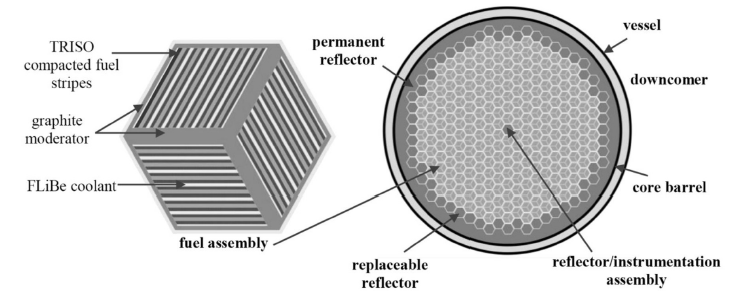
\includegraphics[width=\linewidth]{ahtr.png} 
    \caption{\acrlong{AHTR} fuel assembly (left) and core configuration (right) 
    reproduced from \cite{ramey_monte_2018}.}
    \label{fig:ahtr}
\end{figure}

\subsection{Previous AHTR modeling efforts and challenges} 
\label{sec:previous_ahtr}
\subsubsection{AHTR Neutronics Modeling}
The \gls{AHTR} core design differs significantly from the present \gls{LWR}-based 
nuclear power plants. 
These differences lead to modeling challenges and the need to verify and 
validate simulation methods \cite{ramey_monte_2018}. 
Verification and validation of neutronics and thermal-hydraulics simulation 
capabilities in the context of the \gls{AHTR} design crucially 
support licensure of the \gls{AHTR} design towards the eventual goal 
of deployment \cite{rahnema_phenomena_2019,rahnema_current_2015}. 
Several neutronic studies conducted along the way to the current \gls{AHTR} 
design have shed light on the technical challenges facing the design 
\cite{ramey_monte_2018,holcomb_fluoride_2013,greene_pre-conceptual_2010}. 

The \gls{Georgia Tech} led an Integrated Research Project to 
understand challenges in \gls{AHTR} materials and modeling its neutronics and 
thermal-hydraulics \cite{zhang_integrated_2019}. 
During the research project, a panel of subject matter experts 
generated a \gls{PIRT}.
The \gls{PIRT} identifies areas that need additional research to better 
understand important phenomena for adequate future modeling
\cite{rahnema_phenomena_2019}. 
Table \ref{tab:phenomena} lists the phenomena identified as requiring further 
research. 

\begin{table}[]
    \centering
    \onehalfspacing
    \caption{\acrlong{PIRT} identified \acrlong{AHTR} physical phenomena requiring 
    further research \cite{rahnema_phenomena_2019}.}
	\label{tab:phenomena}
    \footnotesize
    \begin{tabular}{l|l}
    \hline
    \textbf{Category} & \textbf{Phenomena} \\ \hline
    Fundamental cross section data & - Moderation in FliBe \\
    & - Thermalization in FliBe \\
    & - Absorption in FliBe \\
    & - Thermalization in carbon \\
    & - Absorption in carbon \\ \hline
    Material Composition & - Fuel particle distribution \\ \hline
    Computational Methodology & - Solution Convergence \\ 
    & - Granularity of depletion regions \\
    & - Multiple heterogeneity treatment for generating multigroup \\ 
    & cross sections \\
    & - Selection of multigroup structure \\
    & - Boundary conditions for multigroup cross section generation \\ \hline 
    General Depletion & Spectral history \\ \hline 
    \end{tabular}
    \end{table}

The \emph{multiply heterogeneous} \gls{AHTR} fuel, comprised of \gls{TRISO} 
particles embedded in strategically arranged plates, presents simulation challenges. 
We must obtain detailed reference power distributions with individual 
\gls{TRISO} particle fidelity to best understand the \gls{AHTR}'s nuances.
However, deterministic codes that use multigroup cross sections and traditional 
homogenization methods \cite{ramey_monte_2018}, insufficiently capture the 
correct physics in \glspl{AHTR} due to these multiple heterogeneities
\cite{ramey_monte_2018}. 
In the \gls{AHTR}, single and multiple slab homogenization decreased total 
neutron transport simulation time by an order of 10; however, the homogenization 
introduced a nontrivial error of $\sim$3\% \cite{ramey_monte_2018,cisneros_neutronics_2012}.
To determine the feasibility and safety of the \gls{AHTR} design, we must 
calculate core physics parameters to an acceptable uncertainty. 
With Monte Carlo neutron transport, increasing neutron histories reduces statistical 
uncertainty but increases computational cost typically, requiring the use of 
supercomputers to run the simulations.

This \gls{AHTR} presents another technical challenge: the uncertainty of 
graphite moderator material properties: densities, temperatures, and thermal 
scattering data.
Problematically, the thermal scattering data ($S(\alpha,\beta)$ matrices) for 
the bound nuclei in \gls{FLiBe} salts are lacking \cite{ramey_monte_2018}. 
Mei et al. \cite{mei_investigation_2013} and Zhu et al. \cite{zhu_thermal_2017} 
examined the thermal scattering behavior of solid and liquid \gls{FLiBe}.
They concluded that the bound and free atom cross section of \gls{FLiBe} are 
identical above 0.1eV and diverges below 0.01eV, which means that the use or 
absence of thermal scattering data will impact the accuracy of the results 
\cite{ramey_monte_2018}. 

\subsubsection{AHTR Multiphysics Modeling}
In past effort towards multiphysics modeling of the \gls{AHTR}, Gentry et al 
\cite{gentry_development_2016} developed an adapted lattice physics-to-core 
simulator two-step procedure with Serpent \cite{leppanen_serpent_2014} 
and \gls{NESTLE} \cite{turinsky_nestle_1994}. 
The adapted lattice physics-to-core simulator two-step procedure proved to be 
successful for \glspl{LWR} in which few group assembly homogenized group 
constants are generated by 2-D transport lattice calculation and then core 
analysis is performed by 3-D nodal simulation 
\cite{koebke_new_1980,gentry_development_2016}. 
\gls{NESTLE}'s thermal-hydraulics utilizes a \gls{HEM} model for two-phase 
flow and it solves the few-group neutron diffusion equation utilizing the
\gls{NEM} for cartesian and hexagonal reactor geometries.  
Lin \cite{lin_thermal_2020} used RELAP5, a system-level code, to perform 
\gls{AHTR} thermal hydraulics transient simulations to investigate the 
capability of the passive heat removal system. 
In this \gls{AHTR} RELAP5 model, the 252 assemblies are separated into four 
concentric rings and a uniform power distribution is assigned to the fuel 
assemblies in each ring, and more fidelity is placed on the primary and 
\gls{DRACS} system loops. 

\subsection{AHTR Benchmark}
To address and further understand the technical challenges described 
in the previous section, in 2019, the OECD-NEA initiated a benchmark exercise 
to assess the modeling and simulation capabilities for \glspl{AHTR} with 
\gls{TRISO} fuel embedded in fuel planks of hexagonal fuel elements
\cite{noauthor_fluoride_nodate}. 
The benchmark plans to have three phases, starting from a single fuel element 
simulation without burnup, gradually extending to full core depletion and feedback. 
The benchmark's overarching objective is to identify the applicability, accuracy, 
and practicality of the latest methods and codes to assess the current state 
of the art of FHR simulation and modeling \cite{petrovic_preliminary_2021}. 
The benchmark also enables the cross-verification of software and methods 
for the challenging \gls{AHTR} geometry, which is especially useful since 
applicable reactor physics experiments for code validation are scarce 
\cite{petrovic_fhrahtr_2019,petrovic_preliminary_2021}. 
Chapter \ref{chap:fhr-benchmark} will provide a detailed description of the 
benchmark phases and results obtained so far.

\section{Additive Manufacturing}
Additive manufacturing is the formal term for what is popularly known as `3D printing' 
\cite{gibson_additive_2014}. 
The basic principle of additive manufacturing is that a model is initially generated using a
\gls{3D CAD} system and then fabricated directly without the need for process 
planning. 
Additive manufacturing, as the name implies, adds material in layers, such that 
each layer is a thin cross section of \gls{3D CAD}-designed part, as opposed 
to traditional machining which subtracts material instead 
\cite{standard_standard_2012}. 
All commercialized additive manufacturing machines to date use a layer-based approach, and 
the major ways that they differ are in materials, layer creation method, and 
how the layers are bonded to each other \cite{gibson_additive_2014}.
These major differences will determine the: accuracy of the 
final part, material and mechanical properties, the time required to manufacture 
the part, the need for post-processing, the size of additive manufacturing machine, and the overall 
cost of the machine and the process \cite{gibson_additive_2014}. 
Initially, additive manufacturing only manufactured prototypes. 
However, with improvements in material properties, accuracy, and overall quality 
of additive manufacturing output, the applications for additive manufacturing expanded to the 
point at which some industries build parts for direct assembly purposes
\cite{uriondo_present_2015}.  
Furthermore, using additive manufacturing in conjunction with other technologies, such as 
high-power lasers, has enabled additive manufacturing of parts made from various 
metals \cite{gibson_additive_2014}. 

Additive manufacturing has progressed rapidly in the last 30 years, from rapid 
design prototyping with polymers in the automotive industry to scale production 
of metal components.  
Examples include Boeing using additive manufacturing to reduce the 979 
Dreamliner's weight \cite{noauthor_printed_2017} and General Electric using 
additive manufacturing to produce fuel injection nozzles 
\cite{noauthor_transformation_2018}. 
The most common metal additive manufacturing technologies, \gls{SLM}, \gls{EBM}, 
\gls{L-DED}, and binder jetting, are not currently used to manufacture nuclear 
power plant parts. 

The U.S. \gls{DOE}, National Laboratories, \gls{EPRI} support research and 
development efforts towards deployment, testing, and qualification 
of additive manufacturing methods for nuclear components. 
However, the nuclear industry's efforts to incorporate additive manufacturing 
into the supply chain lags behind the auto and aerospace industries due to the 
lack of clarity on regulatory pathways. 
The aerospace and automotive industries benefit from long-standing and resourced 
regulatory and standards development activities \cite{noauthor_roadmap_nodate}. 
Thus, in 2019 the \gls{NRC} addressed these regulatory challenges by issuing 
a draft action plan to prepare the agency to review applications for 
additive manufacturing of nuclear components and clarify the industry's 
expectations of their use \cite{noauthor_roadmap_nodate}.

\subsection{Benefits of Additive Manufacturing for Nuclear Reactor Core Components}
\label{sec:am}
Wide-spread adoption of these methods in the nuclear industry could drastically 
reduce fabrication costs and timelines, combine multiple systems and assembled 
components into single parts, increase safety and performance by tailoring 
local material properties, and enable geometry redesign for optimal load paths 
\cite{simpson_considerations_2019}. 
Many Generation IV advanced reactor concepts have complex geometries, 
such as hex-ducts for sodium-cooled fast reactors, that are costly and difficult 
to fabricate using standard processing techniques. 
Traditional manufacturing routes also restrict many viable geometries for 
reactor designers to explore \cite{sridharan_performance_2019}.  
In summary, reactor core component fabrication with additive manufacturing 
enables further optimization and improvement of fuel geometries to enhance fuel 
performance at lower costs \cite{bergeron_early_2018}. 

\subsection{Demonstration of Additive Manufacturing for Nuclear Reactor Core Components}
Recent nuclear materials experiments have demonstrated the application 
of additive manufacturing to nuclear fuel and structural core material fabrication. 
Rosales et al. \cite{rosales_characterizing_2019} conducted a feasibility study 
of direct routes to fabricate dense uranium silicide (U$_3$Si$_2$) fuel pellets 
using the \gls{INL} approach known as \gls{AMAFT}. 
U$_3$Si$_2$ demonstrates desirable accident-tolerant nuclear fuel properties 
such as high uranium density and improved thermal properties, however, it has 
an expensive and long metallurgical fabrication process. 
Thus, using \gls{AMAFT} to fabricate U$_3$Si$_2$ will lower cost and ensure a
timely and commercially-reliable fabrication process \cite{rosales_characterizing_2019}.  
Sridharan et al. \cite{sridharan_performance_2019} demonstrated the application of
the laser-blown-powder additive manufacturing process to fabricate \gls{FM} steel, a type of 
steel commonly used for cladding and structural components in nuclear reactors. 
Koyanagi et al. \cite{koyanagi_additive_2020} presented the latest 
additive manufacturing technology for manufacturing nuclear-grade \gls{SiC} materials. 
They demonstrated that combinations of additive manufacturing techniques and 
traditional \gls{SiC} densification methods enabled new designs of \gls{SiC} 
components with complex shapes. 
\gls{SiC} demonstrates excellent strength at elevated temperatures, chemical inertness, 
relatively low neutron absorption, and stability under neutron irradiation up 
to high doses \cite{sauder_ceramic_2014, snead_handbook_2007,koyanagi_additive_2020}. 
These qualities make \gls{SiC} suitable for many applications in nuclear systems 
such as fuel cladding, constituents of fuel particles \cite{snead_handbook_2007} 
and pellets \cite{terrani_progress_2015}, and core structural components in fission 
reactors \cite{sauder_ceramic_2014}. 
Trammel et al \cite{trammell_advanced_2019} conducted a preliminary investigation 
to assess the possibilities of fabricating a fuel element with embedded 
\gls{TRISO} fuel using additive manufacturing techniques, such as binderjet printing and \gls{CVI}. 
They successfully demonstrated a fabrication method using the following steps 
(depicted in Figure \ref{fig:ornl-triso-print}): 
\begin{enumerate}
    \item A SiC fuel element structure is first printed with binderjet technology. 
    \item The designated fueled region of the element is loaded with surrogate 
    \gls{TRISO} particles and additional SiC powder to fill interstitial spaces
    between particles. 
    \item The loaded fuel element is densified in a \gls{CVI} process to achieve 
    microencapsulation of \gls{TRISO} particles in a SiC matrix. 
\end{enumerate}
\begin{figure}[]
    \centering
    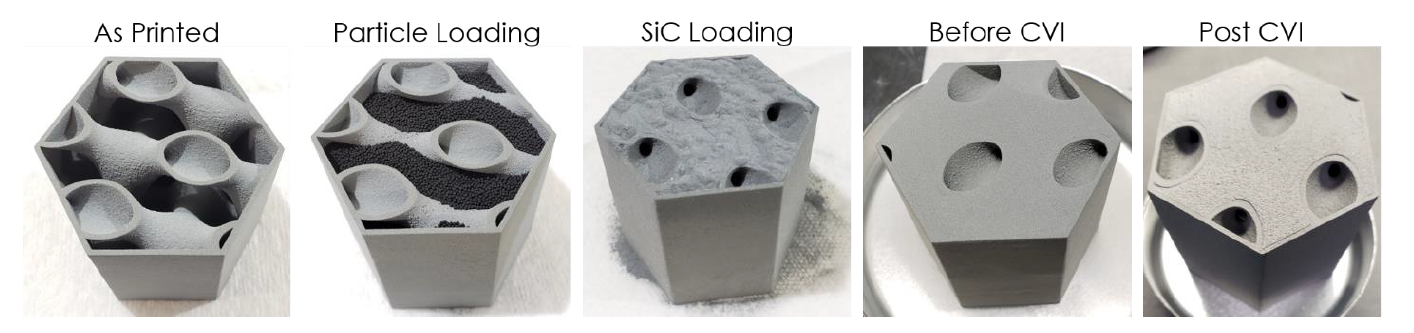
\includegraphics[width=\linewidth]{ornl-triso-print.png} 
    \caption{Stages of additive manufacturing fabrication conducted at \acrlong{ORNL} to 
    produce a fuel element with non-homogenously shaped coolant channels and
    \gls{TRISO} particles embedded in a SiC matrix \cite{trammell_advanced_2019}.}
    \label{fig:ornl-triso-print}
\end{figure}

Many of the materials and fabrication methods discussed are applicable 
for \gls{FHR}-part manufacturing. 
Therefore, this reiterates the possibility of leveraging additive manufacturing to 3D print a
\gls{FHR}-type reactor with non-conventional geometry. 

\section{Nuclear Reactor Design Optimization}
\label{sec:opt}
With the conception of nuclear reactors came along the practice of nuclear 
reactor optimization. 
Nuclear engineering sub-fields such as reactor design, reactor reloading 
patterns, and the nuclear fuel cycle utilize optimization.  
Traditional manufacturing constraints limit nuclear reactor core 
design optimization. 
In the proposed work, we will reexamine nuclear reactor core 
design optimization for arbitrary reactor geometries and fuel distributions
enabled by additive manufacturing. 

\subsection{Previous Efforts for Reactor Design Optimization}
Previous efforts towards reactor design optimization processes utilized 
deterministic and stochastic optimization techniques, coupled with surrogate 
models. 
Deterministic optimization methods usually start from a guess solution.
Then, the algorithm suggests a search direction by applying local 
information to a pre-specified transition rule. 
Any better solution becomes the new solution, and the above procedure continues 
several times \cite{deb_multi-objective_2001}. 
Drawbacks of deterministic methods include: algorithms tend to get stuck at
suboptimal solutions, and an algorithm efficient in solving one type of problem 
may not solve a different problem efficiently \cite{deb_multi-objective_2001}. 
Stochastic optimization methods, such as evolutionary algorithms amd simulated annealing,  
minimize or maximize an objective function when randomness is present. 
Stochasticity enables them to find globally optimal solutions more reliably than 
deterministic methods. 

A nuclear reactor's complexity results in reactor design optimization being a 
multi-objective design problem requiring a tradeoff between desirable 
attributes \cite{byrne_evolving_2014,simon_sciences_2019}. 
When multiple conflicting objectives compete no single optimum solution 
simultaneously optimizes all objectives. 
Instead, multi-objective optimization returns multiple optimal 
solutions that meets each objective to varying degrees \cite{deb_multi-objective_2001}. 
For a multi-objective problem like reactor design, an ideal optimization method 
should find widely spread solutions in the obtained non-dominated front 
\cite{deb_multi-objective_2001}. 
For each solution in a set of non-dominated front solutions, none of 
the objective functions can be improved in value without degrading some of the 
other objective values. 

Recent efforts towards nuclear reactor optimization have relied heavily on 
the aforementioned stochastic methods, with the occasional addition of 
stochastic-deterministic hybrid methods.

\subsubsection{Stochastic Optimization: Simulated Annealing Method}
Simulated annealing iteratively updates one candidate solution until it reaches 
the termination criteria. 
At each iteration, the simulated annealing algorithm selects a random move. 
If the selected move improves the solution, it is always accepted; however,  
if it does not improve the solution, the algorithm updates the solution with 
some probability of less than 1.

Sacco et al. \cite{sacco_two_2006,sacco_metropolis_2008} used stochastic 
simulated annealing and deterministic-stochastic hybrid optimization techniques 
to optimize reactor dimensions, enrichment, materials, etc., to 
minimize the average peaking factor in a three-enrichment-zone reactor. 
Odeh et al. \cite{odeh_core_2016} used the simulated annealing stochastic algorithm 
coupled with neutronics and thermal-hydraulics simulation tools, \gls{PARCS} and RELAP5
\cite{fletcher_relap5mod3_1992}, to develop an optimal \gls{NMR-50} core design 
with a 10-year cycle length and minimal fissile loading. 
Kropaczek et al. \cite{kropaczek_large-scale_2019} demonstrated the constraint 
annealing method: a highly scalable method based on the method of parallel 
simulated annealing with mixing of states \cite{kropaczek_constraint_2019} for 
the solution of large-scale, multiconstrained problems in \gls{LWR} fuel cycle 
optimization. 
These papers demonstrate the simulated annealing optimization method's success in 
reactor design optimization problems. 

Nuclear reactor optimization problems require computationally 
expensive neutronics and thermal-hydraulics software to compute the objective 
function and constraints. 
Multiple papers utilized stochastic optimization methods with surrogate models 
and replace, high-fidelity neutronics or thermal hydraulics 
simulations to reduce computational cost.
Kumar et al. \cite{kumar_new_2015} combined genetic algorithm optimization 
with a surrogate model to optimize for high breeding of $^{233}$U and $^{239}$Pu 
in desired power peaking limits and keff by varying: fuel pin 
radius,  fissile material isotopic enrichment, coolant mass flow rate, and 
core inlet coolant temperature.
Betzler et al. \cite{betzler_design_2019} developed a systematic approach to 
build a surrogate model to serve in place of high-fidelity computational 
analyses. 
They leveraged the surrogate model with a simulated annealing optimization 
algorithm to generate optimized designs at a lower computational cost and
understand the impact of design decisions on desired metrics for \gls{HFIR} \gls{LEU} 
core designs.

The simulated annealing method uses a point-by-point approach:
one solution gets updated to a new solution in one iteration, which does not 
exploit parallel systems' advantages.
Finding an optimal solution with simulated annealing methods takes very 
long if high-fidelity computationally expensive codes are used to compute 
the objective function and constraints.
Therefore, using a simulated annealing method is only practical if a 
surrogate evaluation model is used, as described in Betzler et al. 
\cite{betzler_design_2019} and Kumar et al. \cite{kumar_new_2015}.

\subsubsection{Stochastic Optimization: Evolutionary Algorithm Method}
Peireira et al. \cite{pereira_coarse-grained_2003,pereira_parallel_2008} 
used a coarse-grained parallel genetic algorithm and a niching genetic algorithm
to optimize the same problem as Sacco et al. \cite{sacco_two_2006}. 
Kamalpour et al. \cite{kamalpour_smart_2020} utilized the imperialist competitive 
algorithm, a type of evolutionary algorithm, to optimize a \gls{FCM} fuelled 
\gls{PWR} to extend the reactor core cycle length. 

Contrary to a single solution per iteration in deterministic and stochastic 
simulated annealing methods, evolutionary algorithms use a population of solutions in each 
iteration \cite{deb_multi-objective_2001}. 
Evolutionary algorithm methods mimic nature's evolutionary principles to drive 
the search towards an optimal solution. 
With the affordability and availability of parallel computing systems, the 
evolutionary algorithm optimization method stands out as a method 
that easily and conveniently exploits parallel systems. 
Further, evolutionary algorithms have proved amenable to \gls{HPC} solutions and 
scalable to tens of thousands of processors \cite{kropaczek_constraint_2019}. 
Thus, for optimization problems that require high-fidelity evaluation software, 
the evolutionary algorithm method can leverage parallel computing to find a 
solution faster than the simulated annealing method.
Therefore, in this proposed work, we will utilize the evolutionary algorithm 
optimization method. 

\subsection{Impact of Additive Manufacturing on Nuclear Reactor Design 
Optimization}
Previous efforts toward nuclear reactor optimization, as discussed in the above 
section, focused on optimizing classical reactor parameters such as 
radius of fuel pellet and clad, enrichment of fuel, pin pitch, etc. 
Additive manufacturing advancements for reactor core components remove
conventional fuel manufacturing geometric constraints, allowing the reactor 
designers to optimize beyond classical parameters to enhance fuel performance 
and safety further. 
Reactor design objectives remain consistent with past objectives, such as 
minimizing fuel amount and minimizing the maximum fuel temperature for a given 
power level.
However, we can now approach the nuclear design problems with truly arbitrary 
geometries, no longer limited by traditional geometric shapes that are 
easy to manufacture with traditional processes: slabs as fuel planks, cylinders 
as fuel rods, spheres as fuel pebbles, axis-aligned coolant channels, etc  
\cite{sobes_artificial_2020}.
This has opened the door for a re-examination of reactor core 
optimization in a completely new way, determining the optimal arbitrary geometry 
for a given objective function \cite{sobes_artificial_2020} with a much smaller 
set of constraints. 

With a substantial increase and change in an arbitrary geometry's design space, 
it becomes time consuming for a human reactor designer to thoroughly explore 
and find optimal geometries in the expanded design space. 
Instead, we can leverage \gls{AI} optimization methods (such as evolutionary algorithms) to 
promptly explore the large design space to find global optimal designs. 
\gls{AI} would not replace the human reactor designer but shifts the human 
designer's focus away from conjecturing suitable geometries to defining design 
criteria to find optimal designs \cite{sobes_artificial_2020}. 
Thus, when the human designer changes the reactor criteria, the \gls{AI} 
model will quickly adapt and produce new global optimal designs to fit the new 
criteria.  

\section{Evolutionary Algorithms} 
\gls{AI} research studies `intelligent agents': any device that perceives 
its environment and takes actions that maximize its chance of successfully 
achieving its goals \cite{david_l_poole_computational_1998}.
Evolutionary algorithms, a subset of \gls{AI}, create a population of individual 
solutions, inspired by biological evolution, and induce goals by using a 
`fitness function' to mutate and preferentially replicate high-scoring 
individuals to reach an optimal solution.
Evolutionary algorithms often perform well at approximating solutions to many 
problem types because they do not make any assumptions about the 
underlying fitness landscape.
Genetic algorithms are the most popular evolutionary algorithms for solving 
multi-objective problems \cite{byrne_evolving_2014, krish_practical_2011}. 

\subsection{Genetic Algorithms}
\label{sec:genetic_alg}
Genetic algorithms imitate natural genetics and selection to evolve solutions 
by maintaining a population of solutions, allowing fitter solutions to reproduce
and letting lesser fit solutions die off, resulting in final solutions that are 
better than the previous generations \cite{renner_genetic_2003}. 
From here, we will refer to a solution as an individual within the population. 
genetic algorithms efficiently exploit historical information to speculate new search 
points, improving each subsequent population's performance 
\cite{goldberg_genetic_1989}. 
Genetic algorithms are theoretically and empirically proven to provide robust 
search in complex spaces and are computationally simple yet powerful 
in their search for improvement \cite{goldberg_genetic_1989}. 
Genetic algorithms trounce deterministic and stochastic simulated 
annealing optimization methods, because:
\begin{enumerate}
    \item they search from a population of points
    \item they use objective function information, not derivatives or other 
    auxiliary knowledge of the problem
    \item they use probabilistic transition rules, not deterministic rules
\end{enumerate}
Figure \ref{fig:genetic_alg} depicts the iterative process of using a genetic algorithm
to solve a problem. 
The genetic algorithm generates new populations iteratively until it meets the termination 
criteria. 

\begin{figure}[]
        \centering
        \begin{tikzpicture}[node distance=1.7cm]
                \tikzstyle{every node}=[font=\small]
                \node (1) [lbblock] {\textbf{Create initial population}};
                \node (2) [lbblock, below of=1] {\textbf{Evaluate initial population}};
                \node (3) [lbblock, below of=2, yshift = -1.3cm] {\textbf{Create new population:} \\ 
                \begin{enumerate} \item \textbf{Select} individuals for mating 
                                  \item Create offspring by \textbf{crossover} 
                                  \item \textbf{Mutate} selected individuals 
                                  \item Keep selected individuals from previous generation
                                 \end{enumerate}};
                \node (4) [lbblock, below of=3, yshift=-1.3cm] {\textbf{Evaluate new population}};
                \node (5) [lbblock, below of=4] {\textbf{Is termination \\ criteria satisfied?}};
                \node (6) [lbblock, below of=5] {\textbf{Best solution is returned!}};
                \draw [arrow] (1) -- (2);
                \draw [arrow] (2) -- (3);
                \draw [arrow] (3) -- (4);
                \draw [arrow] (4) -- (5);
                \draw [arrow] (5) -- node[anchor=east] {yes} (6);
                \draw [arrow] (5) -- ([shift={(0.5cm,0cm)}]5.east)-- node[anchor=west] {no} ([shift={(0.5cm,0cm)}]3.east)--(3);
        \end{tikzpicture}
        \caption{Process of finding optimal solutions for a problem with a 
        evolutionary algorithm \cite{renner_genetic_2003}. }
        \label{fig:genetic_alg}
\end{figure}

Genetic algorithms use mechanisms inspired by biological evolution such as selection, 
crossover, and mutation. 
The three operators are simple and straightforward. 
The selection operator selects good individuals. 
The crossover operator recombines good individuals to form a better 
individual. 
The mutation operator alters individuals to create better individuals
\cite{deb_multi-objective_2001}. 
Next, we provide more description and common methods for each operator.

\subsubsection{Selection Operator}
The selection operator duplicates good individuals and eliminates bad individuals 
while keeping the population constant \cite{deb_multi-objective_2001}. 
It achieves this by identifying above-average individuals in a population, 
eliminating bad individuals from the population, and replacing them with 
copies of good individuals.
Selection operator methods utilized in the proposed work include tournament 
selection, best selection, and \gls{NSGA-II} selection. 
In \textit{tournament selection}, a user-defined number of individuals play in 
tournaments, and the best individual proceeds to the next population.
This repeats until all the population's spots are filled. 
In \textit{best selection}, the operator selects a user-defined number of best 
individuals, and copies are made to keep the population size constant. 
In \textit{NSGA-II selection}, the operator selects the best individuals 
from the combination of parent and offspring populations \cite{deb_fast_2002}.
The operator maintains population size by adding copies of the best individuals. 

The selection operator cannot create any new individuals in the population 
and only makes more copies of good individuals at the expense of not-so-good
individuals. 
Instead, crossover and mutation operators perform the creation of new solutions.

\subsubsection{Crossover/Mating Operator}
In most crossover operators, the operator picks two individuals from the population 
at random. 
The operator exchanges some portion of each individuals' attributes with one 
another to create two new individuals \cite{deb_multi-objective_2001}. 
Crossover operator methods utilized in the proposed work include single-point
crossover, uniform crossover, and blend crossover. 
In the single-point crossover, the operator randomly selects two individuals 
from the population and a site along the individual's definition. 
For example, if the individual is a list, the operator randomly chooses an 
element in the list and attributes on this cross site's right side are exchanged 
between the two individuals, creating two new offspring individuals.  
In a uniform crossover, the user defines an independent probability for each 
individual's attribute to be exchanged; usually, $p=0.5$ is used. 
In blend crossover, the operator creates two offspring (O) individuals based on 
a linear combination of two-parent (P) individuals using the following equations: 
\begin{align}
    O_1 &= P_1 - \alpha(P_1-P_2) \\
    O_2 &= P_2 + \alpha(P_1-P_2)
\intertext{where}
\alpha &= \mbox{Extent of the interval in which the new values can be drawn} \nonumber \\
 & \mbox{for each attribute on both side of the parents’ attributes (user-defined)} \nonumber 
\end{align}

The user defines a crossover probability ($p_c$) to preserve some good 
individuals selected during the selection operator stage.  
Therefore, the crossover operator only operates on $100p_c\%$ of the 
population; the rest proceed to the new population \cite{deb_multi-objective_2001}. 
The crossover operator covers the search aspect of the genetic algorithms, 
whereas the mutation operator keeps diversity in the population 
\cite{deb_multi-objective_2001}. 

\subsubsection{Mutation Operator}
The mutation operator alters one or more attributes of an individual within 
a population. 
Mutation occurs in the genetic algorithm based on a user-defined mutation 
probability ($p_m$). 
A low $p_m$ prevents a primitive random search. 
Mutation operator methods utilized in the proposed work include polynomial 
bounded mutation, in which each attribute in each individual is mutated 
based on a polynomial distribution. 
The user also defines each attribute's upper and lower bounds and the 
crowding-degree of the mutation, $\eta$ (a large $\eta$ will produce a mutant 
resembling its parent, while a small $\eta$ will produce the opposite).  

\subsection{Balancing Genetic Algorithm Hyperparameters}
\label{sec:balance}
In the proposed work, hyperparameters refer to parameters whose value controls 
the genetic algorithm's process, such as the population size. 
A well-performing genetic algorithm needs to balance the extent of exploration and 
exploitation; by finding a balance between the conservation of 
valuable individuals obtained until the current generation while exploring new 
individuals. 
With over exploitation of previously obtained individuals, the population loses 
its diversity, resulting in premature convergence to a suboptimal solution. 
Alternatively, if too much stress is given on exploration, the algorithm did not 
appropriately utilize the information obtained thus far, and the genetic 
algorithm's search procedure behaves like a random search process 
\cite{deb_multi-objective_2001}. 
A quantitative balance between these two issues, exploitation and exploration, 
is challenging to achieve. 
Deb et al. \cite{deb_multi-objective_2001} and Goldberg et al. 
\cite{goldberg_toward_1993} quantified the relationship between exploitation 
and exploration. 
They found that for the one-max test problem, in which the objective seeks to 
maximize the number of 1s in a string, a genetic algorithm with any arbitrary 
hyperparameter setting does not work well even on a simple problem. 
Only genetic algorithms with a selection pressure (s) and crossover probability ($p_c$) 
falling inside the control map (Figure \ref{fig:controlmap}) will find the desired 
optimum.  
\begin{figure}[]
    \centering
    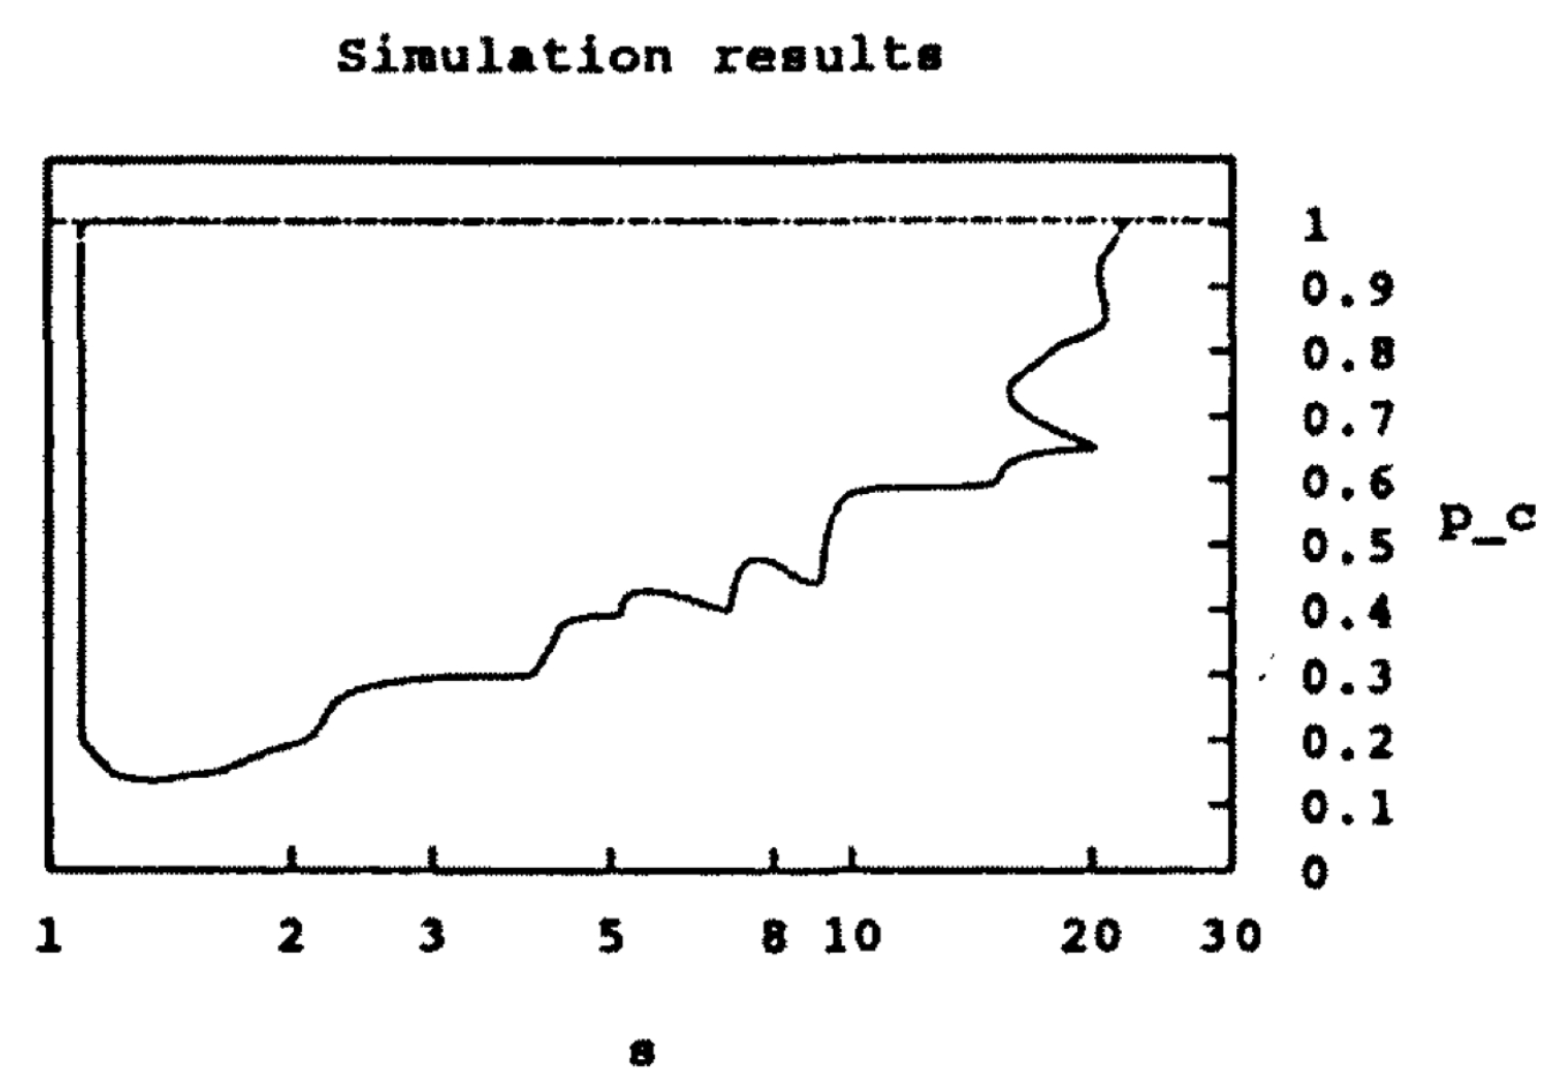
\includegraphics[width=0.6\linewidth]{controlmap.png} 
    \caption{Figure reproduced from \cite{goldberg_toward_1993,deb_multi-objective_2001}
    shows a control map region of selection pressure (s) and crossover probability ($p_c$)
    values in which the genetic algorithm will find the desired optimum for the 
    one-max problem.}
    \label{fig:controlmap}
\end{figure}
Another consideration is the population size. 
A function with considerable variability in objective function values demands 
a large population size to find a global optimum \cite{deb_multi-objective_2001}. 

Therefore, finding an optimized solution with genetic algorithms requires the user 
to conduct a hyperparameter search. 
Ng et al. \cite{ng_improving_2021} suggest that a coarse-to-fine sampling scheme 
is the best way to perform a systematic hyperparameter search.  
For a two-dimensional example of a coarse-to-fine sampling scheme, the user 
first does a coarse sample of the entire square, then a fine search on the 
coarse search's best-performing region. 
Ng et al. also suggests to use random sampling over grid sampling because of the 
former's efficiency in high-dimensional spaces. 
Figure \ref{fig:random_vs_grid_sampling} illustrates how grid sampling gives 
even coverage in the original 2-d space, but provides inefficient coverage in 
projections onto either the x1 or x2 subspace.  
In contrast, random sampling produces a less even distribution in the original 
space, but a far more even distribution in the subspaces.
\begin{figure}[]
    \centering
    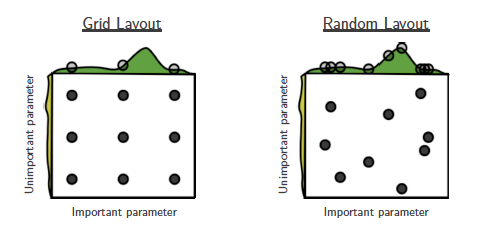
\includegraphics[width=0.8\linewidth]{random_vs_grid_sampling.png} 
    \caption{The impact of grid sampling vs random sampling on coverage of projections 
    into subspaces (reproduced from \cite{}). Random sampling has better coverage 
    in the subspaces.}
    \label{fig:random_vs_grid_sampling}
\end{figure}

\section{Summary}
This chapter provided a literature review of relevant past research 
efforts that give context to this proposed work.
In summary, additive manufacturing of nuclear reactor components is a quickly 
developing field thanks to the aerospace and auto industries, which led to 
breakthroughs in additive manufacturing fabrication of metal components. 
The promise of cheaper and faster manufacturing of reactor components with 
additive manufacturing frees complex reactor geometries from previous manufacturing constraints
and allows reactor designers to reexamine reactor design optimization.  
Stochastic optimization methods such as evolutionary algorithms have proven to 
work well for finding global optimums in multi-objective design problems such as 
nuclear reactor optimization and can be leveraged to explore the vast exploration 
design space enabled by additive manufacturing.